%\section{Preliminaries: Notation and Background}
\section{Background: \Grobner Basis Reduction and Canonical Representations}
\label{sec:prelim}

%This section provides a brief description of the fundamental concepts of: 
%%i) commutative algebra including polynomial rings, polynomial division, ideals, 
% Gr\"obner basis and their application in verification of circuits;
%ii) the algebra of unate cube sets; and iii) the use of ZDDs as an
%implicit set representation for manipulation of Boolean polynomials.

%\subsection{Computer Algebra}

% i.e., $G = GB(J) \Leftrightarrow\  \forall f \in J : f \neq 0 \ \exists g_i \in G :
%lm(g_i)\mid lm(f)$. 

\par Let $\B =\{0,1\}$ denote the Boolean domain, $\F_2$ the finite field
of 2 elements ($\B \equiv \F_2$), and $R = \F_2[x_1, \dots, x_n]$
the  polynomial ring over variables $x_1, \dots, x_n$ with
coefficients in $\F_2$.  
%Since $\Fkk$ is a $k$-dimensional extension of $\F_2$, we
%have that $\Fkk \supset \F_2$ and all $\Fkk (k \geq 1)$ are of
%characteristic 2. 
Operations in $\F_2$ are performed $\pmod{ 2}$, so $-1=+1$ in
$\F_2$. We will use $+ ,\cdot$ to denote addition and multiplication in
$R$, and $\neg, \vee, \wedge$ and $\oplus$ to denote Boolean negation,
OR, AND and XOR operations, respectively. 

A polynomial $f \in R$ is written as a finite sum of terms 
$f = c_1 X_1 +  c_2 X_2 + \dots + c_t X_t$.  Here $c_1, \dots, c_t$
are coefficients and $X_1, \dots, X_t$ are monomials, i.e. power
products of the type $x_1^{e_{1}}\cdot x_2^{e_{2}}\cdots x_n^{e_{n}}$, 
$e_i \in \Z_{\geq  0}$. To systematically manipulate the
polynomials, a monomial order $>$ (also called a term order) is
imposed on the ring. This order $>$ is a total order and a well
order on all the monomials of $R$ such that multiplication by a
monomial preserves the order\footnote{Lexicographic ({\it lex}) and
  degree-lexicographic ({\it deglex}) are examples of such permissible
  monomial orders.}. All polynomials in $R$ are represented using
$>$. Subject to $>$, when a polynomial is written as 
$f = c_1 X_1 +  c_2 X_2 + \dots + c_t X_t$ 
 such that  $X_1 >X_2 > \dots >  X_t$, we call  $lt(f) = c_1 X_1,
 ~lm(f) = X_1, ~lc(f) = c_1$, the {\it leading   term}, {\it   leading
   monomial} and {\it   leading coefficient} of $f$,
 respectively, with $lt(f) = lc(f)\cdot lm(f)$. 
We also denote tail($f$) = $f - lt(f) = c_2X_2 + \dots + c_t X_t$. 
In this work, we are mostly concerned with terms ordered
lexicographically ({\it lex}). 

\begin{Definition} [Boolean Polynomial]
Let $f = c_1 X_1 + \dots + c_t X_t$ be a polynomial in
$\F_2[x_1,\dots,x_n]$ such that the coefficients $c_i \in \{0, 1\}$,
and monomials $X = x_1^{e_{1}}\cdot x_2^{e_{2}}\cdots x_n^{e_{n}}, e_i
\in \{0,1\}$. 
Then $f$ is called a {\bf Boolean polynomial}. For Boolean polynomials
$lt(f) = lm(f)$. 
\end{Definition}

% \textcolor{red}{\begin{Definition} [Pseudo-Boolean Polynomial]
% Let $f = c_1 X_1 + \dots + c_t X_t$ be a polynomial
% such that the coefficients $c_i \in \mathbb{Z}$,
% and monomials $X = x_1^{e_{1}}\cdot x_2^{e_{2}}\cdots x_n^{e_{n}}, e_i
% \in \{0,1\}$. 
% Then $f$ is called a {\bf pseudo-Boolean polynomial}.
% \end{Definition}}

A gate-level circuit can be modeled with Boolean polynomials, where
every Boolean logic gate operator is mapped from $\B$ to a polynomial
function over ${\mathbb{F}}_2$: 

{\small
\begin{equation}
\label{b2poly}
\begin{split}
z ~ =  ~ \neg a ~ & \mapsto ~ z+a+1 \pmod 2  \\
z ~ =  ~ a \wedge b ~ & \mapsto ~ z+a\cdot b \pmod 2\\
z ~ =  ~ a \vee b ~ & \mapsto ~ z+a+b+a\cdot b \pmod 2 \\
z ~ =  ~ a \oplus b ~ & \mapsto ~ z+a+b \pmod 2 
\end{split}
\end{equation}
}

% Using this mapping a Boolean function, say $z = a \vee b$,  
% can be written as the boolean polynomial, $f:z + a\cdot b + a + b$. 
% The solutions to $f = 0$ provide the valid enumerations of  the output and input variables.
%  In this case, $f$ is 0, when $(z,a,b) = \{000,110,101,111\}$  

{\bf Polynomial reduction via division:} Let $f, g$ be polynomials. If
$lm(f)$ is divisible by $lm(g)$, then we say that $f$ {\it is
  reducible to} $r$ modulo $g$, denoted $f
\stackrel{g}{\textstyle\longrightarrow} r$, where $r = f - {lt(f)
  \over   lt(g)} \cdot g$. This operation forms the core operation of
polynomial division algorithms and it has the effect of canceling the
leading term of $f$. 
Similarly, $f$ can be {\it reduced 
w.r.t. a set of polynomials}  $F = \{f_1, \dots, f_s\}$ to obtain a
remainder $r$. This reduction is denoted as $f \stackrel{F} {\textstyle
  \longrightarrow}_+ r$, and the remainder $r$ has the property that
no term in $r$ is divisible (i.e. cannot be canceled) by the leading
term of any polynomial $f_i$ in $F$. Algorithm~\ref{algo:mv_reduce}
(Alg. 1.5.1 from \cite{gb_book}) depicts the procedure to perform this
classical reduction that cancels one monomial in every iteration of
the while-loop.   

\begin{algorithm}[H]
 \caption{Multivariate Reduction of $f$ by $F=\{f_1,\dots,f_s\}$}
 \label{algo:mv_reduce}
 \begin{algorithmic}[1]
 % \Procedure{$multi\_variate\_reduce$}{$f, f_1, \dots, f_s \in \F[x_1, \dots, x_n], f_i\neq 0$}
 \Procedure{$multi\_variate\_reduce$}{$f, \{f_1, \dots, f_s\}, f_i\neq 0$}
 % \ENSURE $u_1,\dots, u_s, r$ s.t. $f = \sum f_i u_i+r$ where $r$ is
 % reduced w.r.t. $F = \{f_1,\dots, f_s\}$ and max($lp(u_1)lp(f_1), \dots, lp(u_s)lp(f_s), lp(r)$) = $lp(f)$
 \State $u_i \gets 0; ~r \gets 0; ~h \gets f $ 
 \While {  $h \neq 0$ }
 \If{ $\exists i$ s.t. $lm(f_i) ~|~ lm(h)$}
 \State choose $i$ least s.t. $lm(f_i) ~|~ lm(h)$
 \State $u_i = u_i + \frac{lt(h)}{lt(f_i)}$
 \State $h = h - \frac{lt(h)}{lt(f_i)} f_i$
 \Else
 \State $r = r+ lt(h)$
 \State $h = h - lt(h)$
 \EndIf
 \EndWhile
 \State \Return $(\{u_1,\dots,u_s\} , r)$
 \EndProcedure
 \end{algorithmic}
 \end{algorithm}

% The algorithm initializes $h$ with the polynomial $f$ and cancels its
% leading term by some  polynomial $f_i \in F$. If the leading term
% $lt(h)$ cannot be canceled by any $lt(f_i)$, then it is added to the  
% remainder $r$ and the process is repeated until all the terms in $h$ are analyzed. 

{\bf Polynomial ideals:} Given a set of polynomials $F = \{f_1, \dots,
f_s\}$ from the ring $R = \mathbb{F}_2[x_1,\dots, x_n]$, the ideal 
generated by $F$ is $J = \langle F\rangle \subseteq R$:
\begin{align}
J = \langle f_1, \dots, f_s \rangle =
\{h_1\cdot f_1+\dots+h_s\cdot f_s: ~h_1,\dots,h_s \in R\},
\end{align}
where the polynomials $f_1,\dots,f_s$ are called the generators (or
basis) of the ideal. 


For a binary variable $x_i$, we have $x_i^2 = x_i$. Therefore, the
polynomial $x_i^2 - x_i$ vanishes over $\Ftwo$, and we call it a
vanishing polynomial. While manipulating Boolean polynomials it is
essential to ensure this indempotency by reducing the polynomials
modulo (the ideal of) all vanishing polynomials $\langle
x_1^2-x_1,\dots,x_n^2-x_n\rangle$. Therefore, %mathematically speaking
we essentially operate on the quotient ring of $\Ftwo[x_1,\dots,x_n]$
modulo the ideal of vanishing polynomials, i.e. %denoted 
over $\Ftwo[x_1,\dots,x_n]/\langle x_1^2-x_1,\dots,x_n^2-x_n\rangle$. 
Then Boolean polynomials are exactly the canonical representatives of
residue classes in the aforementioned quotient ring. A significant
benefit of using a Boolean data-structure such as ZDDs is that the
reduction $x_i^2 = x_i$ is performed implicitly by the
data-structure. 
%, thus improving symbolic computation. Therefore, 
For this reason, in the sequel we {\it omit explicit mention} of
reduction modulo the vanishing polynomials 
% for manipulation of Boolean polynomials, 
and it should be assumed that the reduction $x_i^2 = x_i$
is always performed. 
%It should be clear that in the ZDD-based framework, all
%computations implicitly result in a Boolean polynomial where

{\bf \Grobner basis of ideals:} An ideal $J$ may have many different sets
of generators, i.e. it is possible to have  $J = \langle f_1, \dots,
f_s\rangle = \langle h_1,\dots, h_r\rangle = \dots = \langle g_1,
\dots, g_t \rangle$. A \Grobner basis $G$ of ideal $J$ is one such set
of polynomials $G = GB(J) = \{g_1, \dots, g_t\}$ with many important
properties that allow to solve many polynomial decision questions. 
%A
%\Grobner basis is essentially a canonical representation of the ideal.   

\begin{Definition}[Gr\"obner basis \cite{gb_book}]
\label{def:gb}
%$\bf{\left[Gr\ddot{o}bner\ Basis\right]}$ 
For a monomial ordering $>$, a set  of non-zero polynomials $G =
\{g_1,g_2,\dots,g_t\}$ contained in an ideal $J$, is called a
Gr\"{o}bner basis of $J$ iff 
$\forall f \in J$, $f\neq 0$, there exists $g_i \in 
\{g_1,\dots, g_t\}$ such
that $lm(g_i)$ divides $lm(f)$; i.e., 
$G = GB(J) \Leftrightarrow\  \forall f \in J : f \neq 0, \ \exists g_i \in G :
lm(g_i)\mid lm(f)$. 

\end{Definition}


\par Gr\"obner basis $G$ of an ideal $J = \langle
f_1,\dots,f_s\rangle$ is computed using the Buchberger's
algorithm~\cite{buchberger_thesis}, 
%also given in textbooks \cite{ideals:book} \cite{gb_book}, 
reproduced in Alg. \ref{alg:gb}.

\begin{algorithm}
\caption {Buchberger's Algorithm}
\label{alg:gb}
\begin{algorithmic}[1]
 \Require {$F = \{f_1, \dots, f_s\}$}
 \Ensure  {$G = \{g_1,\dots ,g_t\}$} %, a Gr\"{o}bner basis \\
  \State $G:= F$;
  \Repeat
    \State $G' := G$
    \For {each pair $\{f_i, f_j\}, i \neq j$ in $G'$}
      \State $Spoly(f_i, f_j) \stackrel{G'}{\textstyle\longrightarrow}_+h$ 
      \If {$h \neq 0$} \State $G:= G \cup \{h\}$ \EndIf
    \EndFor
%\hspace{0.2in}  $G(x):=G(x) / x$
  \Until $G = G'$
\end{algorithmic}
\end{algorithm}


% The algorithm initializes the set $G$ with the given generators of $J$
% $i.e.$ $\{f_1,\dots,f_s\}$. Then it takes pairs of polynomials
% ($f_i,f_j$) from the basis and computes their S-polynomial
% $Spoly(f_i,f_j)$:
% algorithm is based on the computation of $Spoly$ of pairwise combination of polynomials 
%in $G$ using the following formula,
In the algorithm,
\begin{equation}
\label{spoly}
\begin{split}
Spoly(f_i,f_j) = \frac{L}{lt(f_i)}\cdot f_i - \frac{L}{lt(f_j)}\cdot f_j
\end{split}
\end{equation}
where $L = LCM(lt(f_i),lt(f_j))$. 
% The $Spoly(f_i,f_j)$ is then reduced
% $w.r.t.$ the polynomials in $G$ to obtain remainder $h$. If $h$ is
% non-zero, it is added to $G$. The process is repeated for all unique
% polynomial pairs, including those generated by the newly added
% elements $h$. The algorithm terminates when there are no new non-zero
% $h$ generated from the set $G$. $Spoly(f_i,f_j)\xrightarrow{G}_+h$
% reductions cancel the leading terms of polynomials $\{f_i,f_j\}$, and
% generate polynomials $h$ with new leading terms, providing additional
% information regarding the ideal.  

An important property of a \Grobner basis $G$ is that reduction of a
polynomial $f$ modulo $G$ is essentially unique. 


\begin{Theorem} [\Grobner Basis Reduction, Thm. 1.9.1 in
      \cite{gb_book}]
\label{thm:gbr}
%$\bf{\left[Gr\ddot{o}bner\ Basis\ Reduction\right]}$ : 
Let $G=\{g_1,\dots,g_t\}$ be a \Grobner basis of ideal $J$, and let $f$
be another polynomial.  The reduction
of $f$ modulo $G$, denoted $f\xrightarrow{G}_+r$, is called the
{\bf \Grobner basis reduction (GBR)} of $f$. The remainder $r$
so obtained by GBR of $f$ is a {canonical expression
modulo $G$}.  
\end{Theorem}

In other words, for {any polynomial} $f$, if $f\xrightarrow{G}_+r_1$
and $f\xrightarrow{G}_+r_2$, then $r_1 = r_2=r$. 
%% The \Grobner basis
%% also provides a decision procedure for ideal membership: To test if
%% any polynomial $f \in J$, we compute $G = 
%% GB(J)$ and check if $f \xrightarrow{G}_+ 0$? 
The remainder $r$ is sometimes also called the {\it normal form} of
$f$ w.r.t. $G$. The canonicity of $r$ (modulo $G$) can be exploited
for equivalence checking of digital circuits. 


%{Verification Formulation}

\begin{Proposition}\label{prop:verif}
Given a circuit $C$, we can represent all the gates using (Boolean)
polynomials $F = \{f_1, \dots, f_s\}$ in $\F_2[x_1,\dots,x_n]$ by
means of Eqn. (\ref{b2poly}), and generate ideal $J  = \langle F \rangle$. Let
$z_i, ~i = 0,\dots,{k-1}, (z_i \in \{x_1,\dots,x_n\})$ denote one-bit of the
$k$-bit primary output variables   
of the circuit.  Compute a \Grobner basis $G = GB(J) =
\{g_1,\dots,g_t\}$ for the polynomials of the circuit, and perform the
GBR $z_i\xrightarrow{G}_+ r_i$ for all $0\leq i<k$. Then all $r_i$'s
are a canonical representation and can be used for formal
verification/equivalence checking. 
\end{Proposition}

To derive the canonical representation $r_i$, it is required to
compute a \Grobner basis $G$ of the ideal generated by the polynomials
of the circuit. Buchberger's algorithm for computation of a Gr\"obner
basis exhibits high complexity. 
% In general, the worst-case \Grobner
% basis complexity is doubly-exponential in the input data
% \cite{Dube:gb-complexity}. However, over ideals that have a finite
% number of solutions, the complexity is single exponentially
% bounded. Particularly 
Over finite fields $\Fq$ of $q$ elements ($q =
2$ in our case), the complexity is bounded by $q^{(O(n))}$, where $n$
is the number of variables \cite{gao:gf-gb-ms}. This complexity still
needs to be overcome. The work of \cite{lv:tcad2013} showed that for
formal verification of combinational circuits, the expensive GB
computation can be avoided altogether, due to the following results. 

\begin{Lemma}[Product Criterion \cite{productc:1979}]
\label{prod_criteria}
%${\bf \left[Product \ Criterion\right]}$ : 
For two polynomials $f_i,f_j$  in any polynomial ring $R$, if the
equality $lm(f_i)\cdot lm(f_j) = LCM(lm(f_i),lm(f_j))$ holds, i.e. if
$lm(f_i)$ and $lm(f_j)$ are relatively prime, then 
$Spoly(f_i,f_j) \xrightarrow{G}_+ 0$.  
\end{Lemma}
 

Using this criterion we can say that when the leading terms of {\it all
polynomials in the basis} $F = \{f_1, \dots, f_s\}$ are relatively
prime, then all $Spoly(f_i,f_j)  \xrightarrow{G}_+ 0$.  As no new
polynomials are generated in Buchberger's algorithm, $F$ is already a
\Grobner basis ($F = GB(J)$). For a combinational
circuit $C$, a specialized term order $>$ can always be derived by
analyzing the circuit topology which ensures such a property
\cite{wienand:cav08} \cite{lv:tcad2013}:  

\begin{Proposition} \label{prop:top-order}
(From \cite{lv:tcad2013}) Let $C$ be an arbitrary combinational
  circuit. Let $\{x_1, \dots, x_n\}$ denote the set of all variables
  (signals) in $C$. Starting from the primary outputs, perform
  a {\it reverse topological traversal} of the circuit and order the
  variables such that $x_i > x_j$ if $x_i$ appears earlier in the
  reverse topological order. Impose a {\it lex} term order $>$ to
  represent each gate as a polynomial $f_i$, s.t. $f_i = x_i +
  tail(f_i)$. Then the set of all polynomials  $\{f_1, \dots, f_s\}$
  forms a Gr\"obner basis G, as $lt(f_i)=x_i$ and $lt(f_j)=x_j$ for
  $i\neq j$ are relatively prime. This term order $>$ is called the 
  {\bf Reverse Topological Term Order (RTTO)}.
\end{Proposition}

Imposition of RTTO on the polynomials of the circuit has the effect of
making every gate output variable $x_i$ a leading term of
$f_i$. Since every gate output is unique, $lm(f_i)=x_i, lm(f_j)=x_j$
become relatively prime. As a result, the set $F$ is already a GB
($G=F$), the explosive GB computation is avoided, and verification is
performed solely by the canonical GB-reduction: $z_i \xrightarrow{G}_+r_i$. 
Note that as $f_i = x_i + \text{tail}(f_i)$, RTTO ensures that
every variable $x_j$ that appears in $\text{tail}(f_i)$ satisfies
$x_i>x_j$. Moreover, the remainder $r_i$ comprises only primary inputs
of the circuit. These properties will be exploited in our algorithms.

% \vspace{-0.1in}
\begin{figure}[!h]
\begin{minipage}[t]{3.25in}
% \vspace{0pt}
\centerline{
%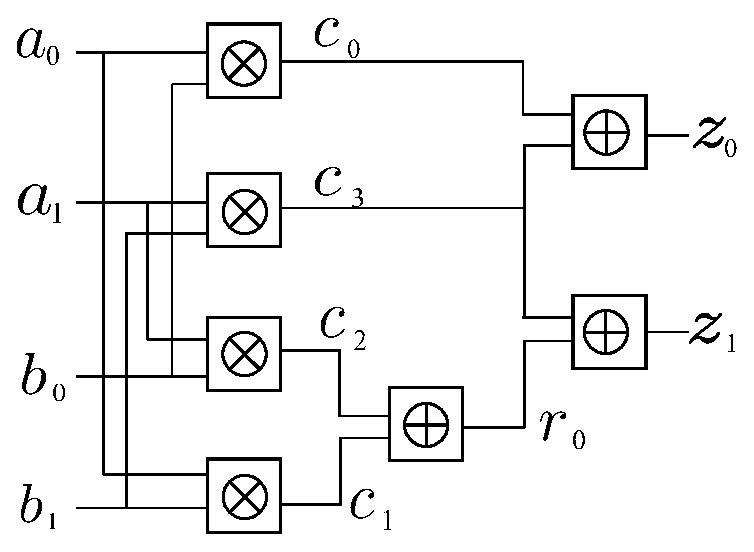
\includegraphics[scale=0.3]{../figures/2bitmultiplier.eps}
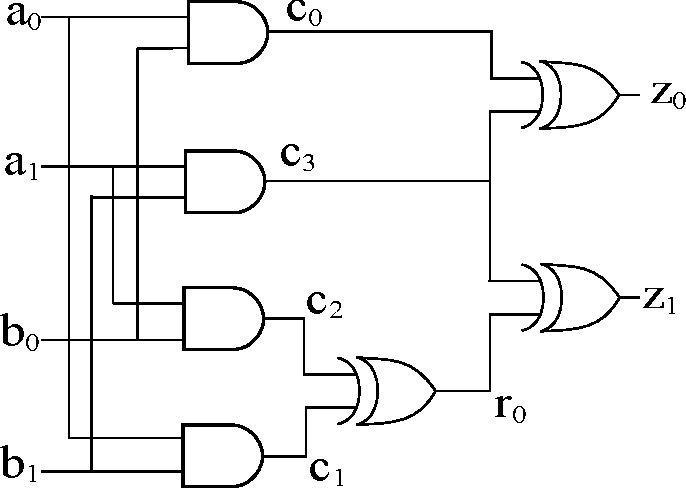
\includegraphics[scale=0.5]{figures/2bitmultiplier_gates.pdf}
}
\caption{\small A 2-bit modulo Multiplier circuit. 
% The gate $\otimes$ is an
%   AND-gate, and $\oplus$ is an XOR-gate; i.e. $\times, +$ modulo 2,
%   respectively.
  } 
\label{fig:mul2bit}
\end{minipage}
\hfill
\begin{minipage}[t]{3.25in}
\vspace{0pt}
%{\small
\begin{align*}
f_1: c_0+a_0 \cdot b_0, \ lm=c_0; ~~~f_2: c_1+a_0 \cdot b_1, \ lm=c_1 \nonumber \\
f_3: c_2+a_1 \cdot b_0, \ lm=c_2; ~~~f_4: c_3+a_1 \cdot b_1, \ lm=c_3 \nonumber \\
f_5: r_0+c_1 + c_2 , \ lm=r_0; ~~~f_6: z_0+c_0 + c_3, \ lm=z_0\nonumber
\end{align*}
\vspace{-0.35in}
\begin{center}
$f_7: z_1+r_0 + c_3, \ lm=z_1$ % \nonumber 
\end{center}
%}
\caption{\small {Polynomials of the circuit under RTTO constitute a GB.
}} 
\label{fig:rel_prime_lt}
\end{minipage}

\end{figure}

%\vspace{-0.1in}
\begin{Example}
\label{ex1}
{\bf Demonstration of the approach:} Consider the circuit given in
Fig. \ref{fig:mul2bit}. 
%Perform a ``reverse topological traversal'' of the circuit. 
Impose RTTO on the circuit. The primary outputs $z_0, z_1$ are both at
level-0, variables $r_0, c_0, c_3$ are at level-1, ~$c_1, c_2$ are at
level-2, and the primary inputs $a_0, a_1, b_0, b_1$ are at
level-3. Order the variables $\{z_0 > z_1\} > \{r_0 > c_0 > c_3\} >
\{c_1 > c_2\} > \{a_0 > a_1 > b_0 > b_1\}$. Using this variable order,
we impose a {\it lex} term order on the monomials. Then all the
polynomials extracted from the circuit have relatively prime leading
terms, as shown in Fig. \ref{fig:rel_prime_lt}, and $G =F = \{f_1, \dots,
f_7\}$ forms a GB. 

Then the GBRs $z_1\xrightarrow{G}_+ a_0\cdot b_0 + a_1\cdot b_1$ and
$z_0\xrightarrow{G}_+a_0\cdot b_1+a_1\cdot b_0 + a_1\cdot b_1$ are
canonical expressions (Boolean polynomials) of the output bits and can
be used for equivalence checking.
\end{Example}


% We will now show how to efficiently implement this GBR
% $z_i\xrightarrow{G}_+r_i$ on circuits by exploiting the implicit set
% representation ZDDs under the imposition of RTTO. 



\section{Unate Cube Sets \& Boolean Polynomials}
\label{sec:unate}

A Boolean {\it variable} represents a dimension of the Boolean space
$\B^n$, and a {\it literal} 
is an instance of a variable $x_i$ or its 
complement $\neg x_i$. A {\it cube} is a product of literals
which denotes a point or a set of points in the Boolean space. A {\it
  cube set} 
consists of a collection of cubes, each of which is a combination of
literals. {\it Unate cube sets} allow for the use of only positive
literals, not negative/complemented literals. 
%Each cube in a unate
%cube set represents a combination, and each literal represents an
%object selected in the combination.

When cube sets are used to represent Boolean functions, they are
usually {\it binate} cube sets containing negative literals. In binate
cube sets, literals $x_i$ and $\neg x_i$ represent $x_i = 1$ and $x_i = 0$,
respectively; while the absence of a literal implies a {\it don't
  care.} In unate cube sets, literal $x_i$ implies $x_i = 1$ whereas
its absence implies $x_i = 0$. For example, the cube set $\{a,
bc\}$ corresponds to points $(abc): \{111, 110, 101, 100, 011\}$ in
the binate cube set representation, whereas it represents $(abc):
\{100, 011\}$ in the unate cube set representation.

Each monomial of a Boolean polynomial can be viewed as a unate cube --
a product of positive literals -- and a Boolean polynomial as a unate
cube set. Then the GBR $z_i\xrightarrow{G}_+ r_i$ can be interpreted
as %(Boolean) algebra 
operations over unate cube sets, 
%resembling a classical logic synthesis problem, 
as shown below. Let us (re)consider the one-step
division for Boolean polynomials: $f\xrightarrow{g} r$. This division
can be interpreted as:



 \begin{align}
\label{eqns:reduce}
f \xrightarrow{g} r & = f - {{lt(f)} \over {lt(g)}} \cdot g \\
& = ~ f - {{lm(f)} \over {lm(g)}} \cdot g; ~~( ~lt(f)=lm(f))\\ 
& = f + {{lm(f)} \over {lm(g)}} \cdot g; ~~~(-1 = +1 \pmod{ 2})\\
& = f \oplus {{lm(f)} \over {lm(g)}} \cdot g; ~~( as ~+ \pmod{2} =
\oplus) \label{eqns:reduce1}
\end{align}



%% {\small
%% \begin{equation}
%% \label{logic_syn}
%% \begin{split}
%% f \xrightarrow{g} r ~  = & ~ f - {{lt(f)} \over {lt(g)}} \cdot g ~ =  ~ f - {{lm(f)} \over {lm(g)}} \cdot g \\
%% = & ~ f + {{lm(f)} \over {lm(g)}} \cdot g ~ =  ~ f \oplus {{lm(f)} \over {lm(g)}} \wedge g
%% \end{split}
%% \end{equation}
%% }

% $$f \xrightarrow{g} r  = f - {{lt(f)} \over {lt(g)}} \cdot g 
% = ~ f - {{lm(f)} \over {lm(g)}} \cdot g; ~~(\text{coeff. 0,1;}
% ~lt(f)=lm(f))
% $$

% $$= f + {{lm(f)} \over {lm(g)}} \cdot g = f \oplus {{lm(f)} \over
%   {lm(g)}} \wedge g \label{eqns:reduce1}
% $$

%We can replace $lt(f)$ with $lm(f)$ as coefficients are either 0 or
%1. 
Notice that ${{lm(f)} \over {lm(g)}}$ is a unate product of 
literals. i.e. a unate cube. The $\oplus$ operation cancels common
cubes from $f$ and ${{lm(f)} \over {lm(g)}}\cdot g$. The $\cdot$
operation models the modulo 2 product, where the partial products are
added using the $\oplus$  operation. Therefore, we
will implement the reduce operation $f\xrightarrow{g} r$ for Boolean
polynomials as $r = f \oplus {{lm(f)} \over {lm(g)}} \cdot g$ using
an implicit representation particularly suited for such unate cube
operations, i.e. ZDDs.  

\subsection{Zero Suppressed Binary Decision Diagrams (ZDDs) for
  Boolean Polynomials}

% A Binary Decision Diagram is a directed graph with two terminal nodes 0 and 1. 
% Each node in the diagram has two edges, solid edge (1-edge) and dotted edge (0-edge). 

Binary decision diagrams (BDDs) \cite{BRYA86} and
their variants 
%such as OKFDDs \cite{drechsler:dac94} and ADDs \cite{add} 
have been used as implicit representations for solving many
Boolean and pseudo-Boolean optimization problems. Zero-suppressed BDDs
\cite{zbdd} are another variant of BDDs that were designed to
efficiently manipulate ``sets of combinations''. A ZDD is obtained
from an ordered BDD by: i) eliminating those vertices whose 1-edge
(then-edge) is incident on the 0-terminal; and ii) merging isomorphic
subgraphs. Subject to the given variable order, a ZDD represents a 
Boolean function canonically. Just as with BDDs, every node in a ZDD
is assigned an index, which corresponds to the variable order imposed
on the diagram. For a detailed description of ZDDs and
their capabilities for solving logic optimization and sparse
combinatorial problems, the reader is referred to \cite{zbdd} and
\cite{zbdd_unate}. 

\begin{figure}[hbt]
\centering
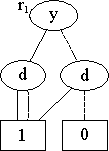
\includegraphics[scale=1]{figures/r1_clean.pdf}
\caption{ZDD for the polynomial $r_1 = yd + y + d$.}
\label{r1}
\end{figure}

In \cite{zbdd_unate}, {\it Minato} demonstrated that ZDDs are an
efficient data-structure for implicit manipulation (algebra) of unate
cube sets. Fig.~\ref{r1} depicts a ZDD for the unate cube set
$\{yd,y,d\}$ with the variable order  $y > d$. The paths beginning
from the root node $y$ and terminating in the 1-terminal node
correspond to the cubes of the set. A variable is present in a cube if
its 1-edge lies on the path; otherwise it is absent from the cube
if its 0-edge lies on the path. 
%Since a monomial of a Boolean
%polynomial is a unate cube, we can interpret a Boolean polynomial as a
%set of unate cubes; and each monomial (cube) as a set of
%variables. 
Consequently, the ZDD of Fig.~\ref{r1} can be construed to
represent the Boolean polynomial $r_1 = yd + y +d$. {\it Minato} has
shown (\cite{zbdd}\cite{zbdd_unate}) how the set union, intersection and
difference operations can be implemented recursively on the ZDDs, 
and they have been implemented using the {\it ite-operator} in
decision diagrams such as the CUDD \cite{cudd} package. We extend
these operations to accommodate the sum and product operations
$\pmod{2}$, i.e. polynomial algebra in $\Ftwo[x_1,\dots,x_n]$, by 
manipulating sets of combinations using ZDDs. 

%, where each unate cube (monomial) represents one combination,
%and each literal represents an object chosen in the combination.
% -- resembling a
%classical logic synthesis problem. 

%Then the ZDD can also be used to represent
%polynomials where the monomials can be obtained the same way the cubes
%are obtained for the equivalent set. 

% Based on the above discussion, we will: i) model GBR as the
% algebra of unate cube sets; ii) use ZDDs as the implicit
% data-structure for this GBR; and iii) devise efficient implementation
% of the GBR by exploiting the special structure imposed by RTTO on the
% ZDD graph.  

%For details on the use of unate cube set algebra in classical logic
%synthesis, and its implementation on ZDDs, we refer the reader to
%\cite{zbdd} \cite{zbdd_unate}. 

